% !TEX root = main.tex

% !TEX root = main.tex

\documentclass[12pt,a4paper]{extarticle}
\usepackage[utf8]{inputenc}
\usepackage[T2A]{fontenc}
\usepackage[russian]{babel}
\usepackage{amsmath, amssymb}
\usepackage{geometry}
\usepackage{hyperref}
\usepackage{graphicx}
\usepackage{microtype}
\usepackage{listings}
\usepackage{xcolor}
\usepackage{setspace}
\usepackage{svg}
\usepackage{float}
\usepackage{subcaption}
\usepackage{embedfile}
\usepackage{indentfirst}
\usepackage{attachfile}

\onehalfspacing
\geometry{top=2cm, bottom=2cm, left=2.5cm, right=1.5cm}

\graphicspath{{img/}}

\begin{document}

\embedfile{../alu_register.v}
\embedfile{../alu_register_tb.v}

\begin{center}
    {\Large \textbf{Домашнее задание по курсу \\ «Введение в архитектуру вычислительных систем»}} \\[0.3cm]
    {\large \textbf{ALU Register} --- вариант 3} \\[1cm]
    
    \textbf{Шелонин Арсений} Б01-411 \\
    \texttt{shelonin.ak@phystech.edu}
\end{center}

\tableofcontents
\newpage

\section{Функциональное описание}

Данное АЛУ выполняет набор инструкций, описанный ниже. Выполняемую на текущем такте инструкцию определяет сигнал с определенного порта. Ширина операндов, внутреннего регистра и шины результата операции определяется параметром модуля \texttt{WIDTH}. АЛУ тактируется положительным фронтом сигнала \texttt{clk\_i}, а также имеет возможность сброса, который (по достижении фронта тактового сигнала) приводит схему в заранее известное состояние: в нашем случае это значение сигнала валидности результата, выставленное в 0, и сохранение результата прошлой операции, так как по ТЗ регистр не сбрасываемый.  

Выполняемые операции:
\begin{table}[h!]
    \begin{tabular}{|l|l|}
        \hline
        \texttt{opcode\_i} & Операция над \texttt{first\_i} и \texttt{second\_i} \\ \hline
        2'b00              & Сложение (знаковое)                                 \\ \hline
        2'b01              & сравнение \texttt{second\_i <= first\_i}            \\ \hline
        2'b10              & Логический сдвиг \texttt{second\_i} влево на \texttt{first\_i} \\ \hline
        2'b11              & Побитовое НЕ-ИЛИ                                    \\ \hline
    \end{tabular}
\end{table}

\section{Структурная схема}
\begin{figure}[H]
    \centering
    \includesvg[width=0.9\textwidth, inkscapelatex=false]{alu}
\end{figure}

\section{Параметры}

\begin{table}[H]
    \begin{tabular}{|l|l|l|}
        \hline
        \textbf{Параметр}  & \textbf{Описание} & \textbf{Допустимые значения}    \\ \hline
        \texttt{WIDTH}     & ширина операндов  & любое натуральное              \\ \hline
    \end{tabular}
\end{table}

\section{Порты}

\begin{table}[H]
    \begin{tabular}{|l|l|l|}
        \hline
        \textbf{Порт}      & \textbf{Ширина} & \textbf{Описание}                \\ \hline
        \texttt{clk\_i}    & 1               & Тактовый сигнал                  \\ \hline
        \texttt{rst\_i}    & 1               & Сигнал сброса                    \\ \hline
        \texttt{valid\_i}  & 1               & Сигнал валидности операции       \\ \hline
        \texttt{first\_i}  & \texttt{WIDTH}  & Шина первого операнда            \\ \hline
        \texttt{second\_i} & \texttt{WIDTH}  & Шина второго операнда            \\ \hline
        \texttt{opcode\_i} & 2               & Шина, кодирующая операцию        \\ \hline
        \texttt{valid\_o}  & 1               & Сигнал валидности результата     \\ \hline
        \texttt{result\_o} & \texttt{WIDTH}  & Шина результата операции          \\ \hline
    \end{tabular}
\end{table}

\section{Тактирование и сброс}
Тактирование осуществляется по положительному фронту сигнала \texttt{clk\_i}. На положительном фронте тактового сигнала при сигнале сброса \texttt{rst\_i} = 1 происходит сброс: \texttt{valid\_o} выставляется в 0. Регистр результата (\texttt{result\_o}) при сбросе не обнуляется и сохраняет свое текущее состояние (либо записывает новые данные из АЛУ, если параллельно выставлен сигнал \texttt{valid\_i} = 1), так как по условию задания он является несбрасываемым

\newpage

\section{Имплементация}
Исходный код модуля: \attachfile{../alu_register.v}

\section{Тестирование}
Исходный код тестировщика: \attachfile{../alu_register_tb.v}

Testbench иллюстрирует весь функционал разрабатываемого модуля. В самом начале происходит сброс. Значения на портах для нового теста выставляются через 1 наносекунду после фронта тактового сигнала, чтобы избежать гонки сигналов. 

\begin{table}[h!]
    \centering
    \begin{tabular}{|l|l|l|l|l|l|}
        \hline
        \textbf{Тест} & \textbf{Действие} & \textbf{valid\_i} & \textbf{opcode\_i} & \textbf{first\_i} & \textbf{second\_i} \\ \hline
        1 & Сложение (знаковое) & 1 & 2'b00 & 8'h0A & 8'h0F \\ \hline
        2 & Сравнение ($second\_i \le first\_i$) & 1 & 2'b01 & 8'hAA & 8'hBB \\ \hline
        3 & Логический сдвиг влево & 1 & 2'b10 & 8'h03 & 8'h0F \\ \hline
        4 & Побитовое НЕ-ИЛИ (NOR) & 1 & 2'b11 & 8'hAA & 8'h55 \\ \hline
        5 & Проверка игнорирования (valid\_i=0) & 0 & 2'b00 & 8'h64 & 8'h64 \\ \hline
    \end{tabular}
\end{table}

\begin{table}[h!]
    \centering
    \begin{tabular}{|l|l|l|l|}
        \hline
        \textbf{Тест} & \textbf{Описание ожидаемого поведения} & \textbf{valid\_o} & \textbf{result\_o} \\ \hline
        1 & $10 + 15 = 25$ & 1 & 8'h19 \\ \hline
        2 & $187 \le 170$ — Ложь (0) & 1 & 8'h00 \\ \hline
        3 & $00001111_2 \ll 3 = 01111000_2$ & 1 & 8'h78 \\ \hline
        4 & $NOT(10101010_2 \ | \ 01010101_2) = 0$ & 1 & 8'h00 \\ \hline
        5 & Запись запрещена (valid\_i=0), сохранение старого значения & 0 & 8'h00 \\ \hline
    \end{tabular}
\end{table}


\begin{figure}[H]
    \centering
    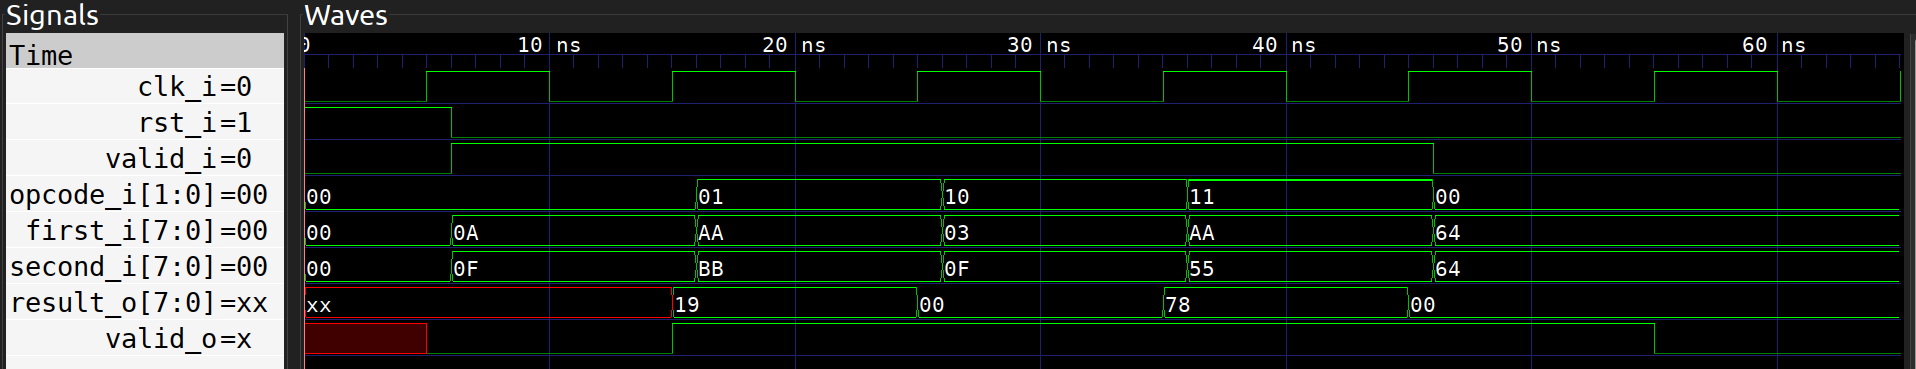
\includegraphics[width=1.0\linewidth]{image.png}
    \caption{\textbf{Результат тестов}}
    \label{fig:placeholder}
\end{figure}
\end{document}